\chapter{Il metodo divide et impera: gli alberi di ricorsione}\label{cap:ricorrenze}

\section{Le ricorrenze}
Nel Capitolo \ref{cap:ricorsione} si è definito il concetto di ricorsione e di metodo divide et impera. Nel metodo \textbf{divide et impera} un problema viene risolto in modo \textbf{ricorsivo}, applicando tre passi ad ogni livello di ricorsione.
\begin{itemize}
	\item \textbf{Divide:} questo passo divide il problema in un certo numero di sottoproblemi che sono istanze più piccole dello \textit{stesso problema}.
	\item \textbf{Impera:} i sottoproblemi vengono risolti in modo \textit{ricorsivo}. Quando si è arrivati ad una dimensione sufficientemente piccola delle istanze, queste vengono risolte direttamente.
	\item \textbf{Combina:} le soluzioni dei sottoproblemi vengono combinate per generare la soluzione del problema generale.
\end{itemize}

Quando i sottoproblemi sono abbastanza grandi da essere risolti ricorsivamente si ha il cosiddetto \textbf{caso ricorsivo}. Una volta che i sottoproblemi diventano sufficientemente piccoli da non richiedere ricorsione si dice che la ricorsione ``ha toccato il fondo'' e che si è raggiunto il \textbf{caso base}. Da notare come tutto questo procedimento abbia come base teorica il \textbf{principio di induzione}.

\dfn{Ricorrenza}{
	Una \textbf{ricorrenza} è un'equazione, detta anche \textbf{equazione di ricorrenza}, che descrive una funzione in termini del suo valore di input con input più piccoli. Una ricorrenza per il tempo di esecuzione di un algoritmo divide et impera si basa sui tre passi del paradigma di base.
}

\begin{example}
	Supposto $T(n)$ sia il tempo di esecuzione di un problema di dimensione $n$. Se la dimensione del problema è sufficientemente piccola, per esempio $n \leq c$ per qualche costante $c$, la soluzione diretta richiede un tempo costante, che si indica con $\Theta(1)$. Supposto che la suddivisione del problema generi $a$ sottoproblemi e che la dimensione di ciascun sottoproblema sia $1/b$ volte la dimensione del problema originale allora servirà tempo $T(n/b)$ per risolvere un sottoproblema di dimensione $n/b$ e quindi, per risolverne $a$, servirà un tempo $a \cdot T(n/b)$. Se impieghiamo un tempo $D(n)$ per dividere il problema in sottoproblemi e un tempo $C(n)$ per combinare le soluzioni dei sottoproblemi nella soluzione del problema originale, si ottiene la ricorrenza:
\begin{displaymath}
	T(n)=
	\begin{cases}
		\Theta(1) & \text{se } n\leq c \\
		aT(n/b)+D(n)+C(n) & \text{negli altri casi}
	\end{cases}
\end{displaymath}
\end{example}

I sottoproblemi non devono necessariamente essere espressi mediante una frazione costante della dimensione del problema iniziale. Ad esempio, una versione ricorsiva della ricerca lineare all'interno di un array non creerebbe un solo sottoproblema in quanto dovrebbe richiamare sé stessa, fino a quando l'elemento da ricercare non è stato trovato, su un array contenente un elemento in meno rispetto alla chiamata padre. La ricorrenza che si ottiene sarà allora:
\begin{displaymath}
	T(n) = \begin{cases}
		\Theta(1) & \text{se } n=1\\
		T(n-1)+\Theta(1) & \text{se } n>1
	\end{cases}
\end{displaymath}

\section{Metodo dell'albero di ricorsione}
In un \textbf{albero di ricorsione} ogni nodo rappresenta il costo di un singolo sottoproblema da qualche parte nell'insieme delle chiamate ricorsive di funzione. Sommando i costi all'interno di ogni livello dell'albero è possibile determinare il costo totale di un algoritmo ricorsivo. Questa analisi prende il nome di \textbf{metodo dell'albero di ricorsione}.

\begin{example}
	Si consideri l'equazione:
\begin{equation}\label{eqricorrenza1}
	T(n)=
	\begin{cases}
		\Theta(1) & \text{se } n \leq 1 \\
		2T(n/2)+ \Theta(n) & \text{se } n >1
	\end{cases}
\end{equation}
\end{example}

Data l'equazione~\ref{eqricorrenza1} è possibile costruire l'albero di ricorsione come mostrato di seguito. Ogni nodo interno rappresenta l'input di una chiamata ricorsiva.
\begin{center}
\begin{forest}
[$n$
	[$\frac{n}{2}$
		[$\frac{n}{4}$
			[$\frac{n}{8}$
				[$1$,edge=dashed]
				[$1$,edge=dashed]
			]
			[$\frac{n}{8}$
			[$1$,edge=dashed]
			[$1$,edge=dashed]
			]
		]
		[$\frac{n}{4}$
		[$\frac{n}{8}$
		[$1$,edge=dashed]
		[$1$,edge=dashed]
		]
		[$\frac{n}{8}$
		[$1$,edge=dashed]
		[$1$,edge=dashed]
		]
		]
	]
	[$\frac{n}{2}$
	[$\frac{n}{4}$
	[$\frac{n}{8}$
	[$1$,edge=dashed]
	[$1$,edge=dashed]
	]
	[$\frac{n}{8}$
	[$1$,edge=dashed]
	[$1$,edge=dashed]
	]
	]
	[$\frac{n}{4}$
	[$\frac{n}{8}$
	[$1$,edge=dashed]
	[$1$,edge=dashed]
	]
	[$\frac{n}{8}$
	[$1$,edge=dashed]
	[$1$,edge=dashed]
	]
	]
	]
]
\end{forest}
\end{center}

Poiché le dimensioni dei sottoproblemi si dimezzano ogni volta che si scende di un livello, alla fine si dovrà raggiungere una condizione al contorno rappresentata dalle foglie dell'ultimo livello. A quale distanza dalla radice si trovano le foglie? La dimensione del sottoproblema per un nodo alla profondità $i$ è $n/2^{i}$. Quindi, la dimensione del sottoproblema diventa $1$ quando \[ \frac{n}{2^{i}}=1\]

ovvero quando \[n=2^{i}\]

cioè \[i=\log_{2}n\]

Dunque l'albero ha $\log_{2}n+1$ livelli. Possiamo determinare inoltre il costo a ogni livello dell'albero. Ogni livello ha due volte i nodi del livello precedente; quindi il numero di nodi alla profondità $i$ è $2^{i}$.

Poiché le dimensioni dei sottoproblemi diminuiscono di un fattore 2 ogni volta che si scende di un livello rispetto alla radice, ogni nodo alla profondità $i$ (per $i= 0, 1, 2, ..., \log_{2}n-1$) ha un costo di $(n/2^{i})$. Moltiplicando il costo di ciascun nodo per il numero di nodi su ogni livello si ottiene che il costo, livello per livello, di tutti i nodi interni è esattamente $\Theta(n)$. L'ultimo livello, all'altezza $\log_{2}n$, ha $2^{\log_{2}n}=n^{\log_{2}2}=n$ nodi, ciascuno con un costo $T(1)$, per un costo totale pari a $nT(1)$ che è $\Theta(1)$, in quanto supponiamo che $T(1)$ sia una costante.

A questo punto sommiamo i costi di tutti i livelli per determinare il costo dell'albero intero:
\begin{eqnarray*}
	T(n) &=& \sum_{i=0}^{\log_{2}n}\Theta(n)+\Theta(1) \nonumber \\
	&=& \log_{2}n \cdot \Theta(n)+\Theta(1) \nonumber \\
	&=&\Theta(n\log_{2}n)
\end{eqnarray*}
\pagebreak
\begin{example}
	Si consideri la funzione fattoriale $n!$. Il \textit{fattoriale} di un numero naturale $n$ può essere definito sia mediante un approccio iterativo che in maniera ricorsiva. Si dimostra infatti grazie al principio di induzione che:
\begin{displaymath}
	n!=
	\begin{cases}
		1 & \mbox{se } n=1\\
		n(n-1)! & \mbox{se } n>1
	\end{cases}
\end{displaymath}
\end{example}

Il tempo di esecuzione per il calcolo del fattoriale può essere espresso tramite la seguente equazione di ricorrenza:
\begin{equation}\label{eq:fattoriale}
	T_{F}(n)=
	\begin{cases}
		\Theta(1) & \mbox{se } n =1 \\
		T_{F}(n-1)+\Theta(1) & \mbox{se } n>1
	\end{cases}
\end{equation}
che può essere rappresentato mediante un albero di ricorsione degenere:
\begin{center}
	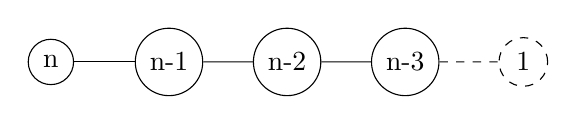
\begin{tikzpicture}
		[node/.style={circle,draw,minimum size=0.5cm},rotate=90]
		\node[node]{n}
		child{
			node[node]{n-1}
			child{
				node[node]{n-2}
				child{
					node[node]{n-3}
					child[dashed]{node[node]{1}}
				}
			}
		};
	\end{tikzpicture}
\end{center}

Per ogni nodo conosciamo il \textit{contributo locale} dato da $\Theta(1)$ mentre si vede facilmente che l'altezza totale dell'albero è esattamente $n$. Il costo sarà quindi:
\begin{eqnarray*}
	T_{F}(n) &=& \sum_{i=0}^{n-1} \Theta(1) + \Theta(1) \nonumber \\
	&=& (n-1)\cdot \Theta(1) + \Theta(1) \nonumber \\
	&=& n \cdot \Theta(1) \nonumber \\
	&=& \Theta(n)
\end{eqnarray*}

\subsection{Forma generale delle equazioni di ricorrenza}

\gbox{Forma generale delle equazioni di ricorrenza}{green-gradient-4}{
	La \textbf{forma generale delle equazioni di ricorrenza con un solo parametro} è del tipo:
\begin{equation}\label{eq:forma_generale_ricorrenza}
	T(n) =
	\begin{cases}
		\Theta(1) & \text{se } n \leq k \\
		\sum_{i=1}^{Z(n)} T(f_{i}(n)) + g(n) & \text{se } n > k \\
	\end{cases}
\end{equation}
Dove:
\begin{itemize}
	\item $Z(n)$ è il \textbf{numero di chiamate ricorsive} esprimibile come funzione di $n$;
	\item Le funzioni $f_{i}(n)$ rappresentano le dimensioni dell'input dei sottoproblemi;
	\item Deve essere $f_{i}(n)<n$ per garantire la \textbf{convergenza} del metodo induttivo;
	\item La funzione $g(n)$ rappresenta il \textbf{contributo locale};
\end{itemize}
}

\begin{osservation}
	Al variare della funzione $Z(n)$ varierà la forma dell'albero di ricorrenza. Infatti, sia $T(n)=\sqrt[]{n} \cdot T(\sqrt[]{n})$. Questa equazione genererà un albero dove ogni livello avrà $\sqrt[]{n}$ volte la dimensione dell'input: al primo livello saranno quindi $\sqrt{n}$ nodi mentre al secondo $\sqrt{n} \cdot(\sqrt{\sqrt{n}})$ nodi e così via generando quello che si dice un \textbf{albero variabile}.

\end{osservation}

\begin{example}
	Sia
\begin{displaymath}
	T(n) =
	\begin{cases}
		1 & \mbox{ se } n \leq 1 \\
		2T(n/4) +n^{2} & \mbox{ se } n > 1 \\
	\end{cases}
\end{displaymath}
\end{example}

Volendo esprimere l'equazione della ricorrenza come l'abbiamo vista nella forma generale sarà:
\begin{displaymath}
	\sum_{i=1}^{2}T(n/4) + n^{2}
\end{displaymath}
Dove $z(n)=2$, $g(n)=n^{2}$, $f_{i}(n)=n/4$. Il coefficiente 2 ci dice che l'albero generato sarà \textit{binario}.

I passi per risolvere questa equazione saranno quindi i seguenti:
\begin{enumerate}
	\item \textbf{Disegno dell'albero binario:}
	\begin{center}
\begin{forest}
	[$n$
		[$\frac{n}{4}$
			[$\frac{n}{16}$
				[$\frac{n}{32}$
					[$1$,edge=dashed]
					[$1$,edge=dashed]
				]
				[$\frac{n}{32}$
				[$1$,edge=dashed]
				[$1$,edge=dashed]
				]
			]
			[$\frac{n}{16}$
				[$\frac{n}{32}$
					[$1$,edge=dashed]
					[$1$,edge=dashed]
				]
				[$\frac{n}{32}$
				[$1$,edge=dashed]
				[$1$,edge=dashed]
				]
			]
		]
		[$\frac{n}{4}$
			[$\frac{n}{16}$
				[$\frac{n}{32}$
					[$1$,edge=dashed]
					[$1$,edge=dashed]
				]
				[$\frac{n}{32}$
				[$1$,edge=dashed]
				[$1$,edge=dashed]
				]
			]
			[$\frac{n}{16}$
				[$\frac{n}{32}$
					[$1$,edge=dashed]
					[$1$,edge=dashed]
				]
				[$\frac{n}{32}$
				[$1$,edge=dashed]
				[$1$,edge=dashed]
				]
			]
		]
	]
\end{forest}
	\end{center}
	\item \textbf{Estrapolazione della relazione tra il livello e il numero dei nodi.} Se: $$f_{i} = f_{j} \quad \forall i,j \ (1 \leq i, j \leq z(n))$$ allora tutti i nodi prendono lo stesso input. In questo caso: $f_{i}=n/4 \quad \forall \ i (1 \leq i \leq 2)$ e ad ogni livello si ha che il \textbf{termine generale} è $\dfrac{n}{4^{i}}$
	\item \textbf{Associazione del costo di ogni livello:} ciascun nodo ha un costo quadratico rispetto all'input che ricevono, questo ci è dato dall'informazione sul contributo locale presente nell'equazione di ricorrenza. Oltre a questo, ogni livello ha $2^{i}$ nodi essendo un albero binario. Questo significa che la somma dei nodi su ciascun livello sarà dato da:
	\begin{displaymath}
	2^{i}\Bigl(\frac{n}{4^{i}}\Bigl)^{2}
	\end{displaymath}
	che può essere riscritto come:
	\begin{eqnarray*}
	2^{i}\Bigl(\frac{n}{4^{i}}\Bigl)^{2} &=& n^{2} \cdot \frac{2^{i}}{4^{2i}} \\
	&=& n^{2} \cdot 2^{i-4i}\\
	&=& n^{2} \cdot 2^{-3i} \\
	&=& \frac{n^{2}}{2^{3i}}\\
	\end{eqnarray*}

	\item \textbf{Calcolo dell'altezza dell'albero cercando il livello delle foglie.} Per ottenere delle foglie bisogna raggiungere il caso base. Quindi:
	\begin{displaymath}
	\frac{n}{4^{i}}=1 \Leftrightarrow n=4^{i} \Leftrightarrow i= \log_{4} n \Leftrightarrow i=\frac{\log_{2}n}{2}
	\end{displaymath}
	\item \textbf{Calcolo i contributi delle foglie:} nel caso di \textbf{alberi pieni} le foglie si trovano tutte sullo \textit{stesso livello}\footnote{In generale quando le funzioni $f_{i}$ sono diverse non ci troveremo davanti ad alberi pieni e sarà impattante nel calcolo del costo generale.}. Nel caso di questa equazione ci troviamo davanti ad un albero pieno in quanto la funzione $f_{i}$ è unica e il suo termine decresce in maniera quadratica.

	Se l'altezza è $h= \frac{\log_{2}n}{2}$ il numero delle foglie sarà $2^{h}$, ovvero:
	\begin{eqnarray*}
	2^{h} &=& 2^{\frac{\log_{2}n}{2}} \\
	&=&  2^{\frac{1}{2}}\cdot \log_{2}n) \\
	&=& (2^{\log_{2}n})^{ \frac{1}{2}} \\
	&=& \sqrt{n} \\
	\end{eqnarray*}
	\item \textbf{Calcolo del costo totale: } Si somma il costo delle foglie che sarà $1 \cdot \sqrt{n} = \sqrt{n}$ per il costo dei nodi interni.
	\begin{displaymath}
	\sqrt{n}+ \sum_{i=0}^{h-1} (\frac{n^{2}}{8^{i}}) = \sqrt{n}+\sum_{i=0}^{\frac{\log_{2}n}{2}-1} \bigl( \frac{n^{2}}{8^{i}} \bigl)\\
	\end{displaymath}
	Portando fuori dalla sommatoria il termine $n^{2}$ si ottiene:
	\begin{displaymath}
	\sqrt{n}+n^{2}\cdot \sum_{i=0}^{\frac{\log_{2}n}{2}-1} \bigl( \frac{1}{8^{i}} \bigl)
	\end{displaymath}
	Ottenendo così una \textit{serie geometrica}. Notiamo inoltre che la \textit{ragione} della serie geometrica è minore di quindi, questo garantisce che la serie:
	\begin{displaymath}
	\sum_{i=0}^{\infty}(\frac{1}{8})^{i}
	\end{displaymath}
	converge e in particolare la sua somma vale:
	\begin{displaymath}
	\frac{1}{1-\frac{1}{8}}= \frac{8}{7}
	\end{displaymath}
	Quindi possiamo dire in generale che, data una serie geometrica convergente vale:
	\begin{displaymath}
	\underbrace{\sum_{i=0}^{0} x^{i}}_{\Theta(1)} \leq \sum_{i=0}^{z} x^{i} \leq \underbrace{\sum_{i=0}^{\infty} x^{i}}_{\Theta(1)} = \frac{1}{1-x}
	\end{displaymath}
	Quindi:
	\begin{displaymath}
	\sqrt{n}+n^{2}\cdot \underbrace{\sum_{i=0}^{\frac{\log_{2}n}{2}-1} \bigl( \frac{1}{8^{i}} \bigl)}_{\Theta(1)} = \Theta(\sqrt{n}+n^{2}) = \Theta(n^{2})
	\end{displaymath}
\end{enumerate}

\begin{example}
	Sia
\begin{displaymath}
	T(n)=
	\begin{cases}
		1 & \mbox{se } n \leq 2\\
		3 \cdot T(\sqrt{n}) + 1 & \mbox{se } n>2 \\
	\end{cases}
\end{displaymath}
\end{example}

Nella nostra analisi la funzione $f_{i}(n)$ mette in relazione la dimensione dell'input tra nodo padre e nodo figlio. Quindi in particolare indica la \textit{velocità della decrescita}. Più veloce sarà più basso sarà l'albero di ricorrenza. Essendo unica la funzione è garantito il fatto che abbiamo a che fare con un albero pieno dove ogni nodo genera tre nodi figli.
\begin{center}
\begin{forest}
	for tree ={
		scale = 0.7
	}
[$n$
	[$n^{\frac{1}{2}}$
		[$n^{\frac{1}{4}}$
			[$n^{\frac{1}{8}}$]
			[$n^{\frac{1}{8}}$]
			[$n^{\frac{1}{8}}$]
		]
		[$n^{\frac{1}{4}}$
		[$n^{\frac{1}{8}}$]
		[$n^{\frac{1}{8}}$]
		[$n^{\frac{1}{8}}$]
		]
		[$n^{\frac{1}{4}}$
		[$n^{\frac{1}{8}}$]
		[$n^{\frac{1}{8}}$]
		[$n^{\frac{1}{8}}$]
		]
	]
	[$n^{\frac{1}{2}}$
	[$n^{\frac{1}{4}}$
	[$n^{\frac{1}{8}}$]
	[$n^{\frac{1}{8}}$]
	[$n^{\frac{1}{8}}$]
	]
	[$n^{\frac{1}{4}}$
	[$n^{\frac{1}{8}}$]
	[$n^{\frac{1}{8}}$]
	[$n^{\frac{1}{8}}$]
	]
	[$n^{\frac{1}{4}}$
	[$n^{\frac{1}{8}}$]
	[$n^{\frac{1}{8}}$]
	[$n^{\frac{1}{8}}$]
	]
	]
	[$n^{\frac{1}{2}}$
	[$n^{\frac{1}{4}}$
	[$n^{\frac{1}{8}}$]
	[$n^{\frac{1}{8}}$]
	[$n^{\frac{1}{8}}$]
	]
	[$n^{\frac{1}{4}}$
	[$n^{\frac{1}{8}}$]
	[$n^{\frac{1}{8}}$]
	[$n^{\frac{1}{8}}$]
	]
	[$n^{\frac{1}{4}}$
	[$n^{\frac{1}{8}}$]
	[$n^{\frac{1}{8}}$]
	[$n^{\frac{1}{8}}$]
	]
	]
]
\end{forest}
\end{center}
Il termine generale dei nodi per ciascun livello sarà dato da:
\begin{displaymath}
	n^{\frac{1}{2^{i}}}
\end{displaymath}
Dove ciascun nodo contribuisce in modo costante. Il costo di ciascun livello sarà quindi:
\begin{displaymath}
	3^{i}
\end{displaymath}
Per trovare l'altezza si pone
\begin{displaymath}
	n^{\frac{1}{2^{i}}}=2
\end{displaymath}
Applicando il logaritmo si ottiene:
\begin{eqnarray*}
	\log_{2}n^{\frac{1}{2^{i}}} &=& \frac{1}{2^{i}} \cdot \log_{2} n\\
	&=& 1 \\
	&\Leftrightarrow & \log_{2} n = 2^{i} \\
	&\Leftrightarrow & \log_{2}(\log_{2}n) = i
\end{eqnarray*}
Le foglie saranno quindi:
\begin{displaymath}
	3^{\log_{2}(\log_{2}n)}
\end{displaymath}
Quindi il costo dell'equazione di ricorrenza sarà:
\begin{eqnarray*}
	T(n) &=& \sum_{i=0}^{\log_{2}(\log_{2}n))-1} 3^{i} + 3^{\log_{2}(\log_{2}n)} \\
	&=& (\log_{2}n)^{\log_{2}3}+\sum_{i=0}^{\log_{2}(\log_{2}n))-1} 3^{i}\\
	&=& (\log_{2}n)^{\log_{2}3} + \frac{3^{\log_{2}(\log_{2}n)}-1}{2}\\
	&=& (\log_{2}n)^{\log_{2}3} + \frac{(\log_{2}n)^{\log_{2}3}-1}{2}\\
	&=& \frac{2(\log_{2}n)^{\log_{2}3}+(\log_{2}n)^{\log_{2}3}-1}{2}\\
	&=& \frac{3(\log_{2}n)^{\log_{2}3}-1}{2}\\
	&=& \Theta((\log_{2}n)^{\log_{2}3})
\end{eqnarray*}
Consideriamo l'equazione
\begin{displaymath}
	T(n)=
	\begin{cases}
		1 & \mbox{se } n \leq 1\\
		T(n/2)+T(n/3)+n & \mbox{se } n> 1\\
	\end{cases}
\end{displaymath}
In questo esempio abbiamo due funzioni:
\begin{displaymath}
	f_{1}(n)=\frac{n}{2} \qquad f_{2}(n)=\frac{n}{3}
\end{displaymath}
Scriviamo l'albero di ricorrenza:
\begin{center}
\begin{forest}
[$n$
	[$\frac{n}{2}$
		[$\frac{n}{4}$
			[$\frac{n}{8}$
				[$\frac{n}{16}$
					[$\frac{n}{32}$]
					[$\frac{n}{48}$]
				]
				[$\frac{n}{24}$]
			]
			[$\frac{n}{12}$
				[$\frac{n}{24}$]
				[$\frac{n}{36}$]
			]
		]
		[$\frac{n}{6}$
			[$\frac{n}{12}$]
			[$\frac{n}{18}$]
		]
	]
	[$\frac{n}{3}$
		[$\frac{n}{6}$
			[$\frac{n}{12}$]
			[$\frac{n}{18}$]
		]
		[$\frac{n}{9}$
			[$\frac{n}{18}$]
			[$\frac{n}{27}$]
		]
	]
]
\end{forest}
\end{center}
A differenza di un albero pieno, in questo caso esistono rami più veloci e rami più lenti. Questo perché le espressioni che corrispondono alle dimensioni dell'input sono diverse. L'albero che ne esce non sarà quindi pieno: ci saranno rami che arriveranno più lentamente alle foglie mentre altri avranno una profondità molto piccola.

In casi del genere, associato il contributo di ogni nodo e capito il termine generale per ogni livello, si calcola il costo dei due alberi pieni relativi all'altezza del ramo più veloce e del ramo più lento. Il costo dell'albero sarà compreso tra questi due limiti, uno \textit{inferiore} e uno \textit{superiore}. Si procede quindi per \textbf{approssimazione}.

Per il primo albero si usa la lunghezza del ramo più veloce, ovvero i termini che decrescono seguendo la successione: $$\frac{n}{3},\frac{n}{9},\frac{n}{27},\ldots$$ È chiaro che il termine generale, livello dopo livello, è: $$\frac{n}{3^{i}}$$Ciò significa che l'altezza dell'albero sarà:$$\frac{n}{3^{i}}=1 \implies n=3^{i} \iff \log_{3}n=i$$

Per il secondo albero useremo la lunghezza del ramo più lento, ovvero i termini che decrescono seguendo la successione: $\frac{n}{2}, \frac{n}{4}, \frac{n}{8},...$. Il termine generale sarà:$$\frac{n}{2^{i}}$$ e l'altezza dell'albero sarà:$$\frac{n}{2^{i}}=1 \implies i=\log_{2}n$$

Per ogni livello il contributo dato dalla somma dei nodi è:
\begin{itemize}
	\item \textbf{Livello 1:} $\frac{n}{2}+\frac{n}{3}=\frac{5n}{6}$
	\item \textbf{Livello 2:} $\frac{n}{4}+\frac{n}{6}+\frac{n}{6}+\frac{n}{9}=\frac{25}{36}n=(\frac{5}{6})^{2}n$
	\item \textbf{Livello 3:} $\frac{n}{8}+\frac{n}{12}+\frac{n}{12}+\frac{n}{8}+\frac{n}{12}+\frac{n}{18}+\frac{n}{18}+\frac{n}{27}=\frac{125}{216}n=(\frac{5}{6})^{3}n$
\end{itemize}
Si ottiene quindi che il termine generale, livello dopo livello sarà dato da: $$(\frac{5}{6})^{i}n$$
A questo punto si possono calcolare le due sommatorie:
\begin{displaymath}
	T'(n)=\sum_{i=0}^{\log_{3}n}\Bigl(\frac{5}{6}\Bigl)^{i}n
\end{displaymath}
e
\begin{displaymath}
	T''(n)=\sum_{i=0}^{\log_{2}n}\Bigl(\frac{5}{6}\Bigl)^{i}n
\end{displaymath}
Sarà quindi:
\begin{eqnarray*}
	T'(n)&=&\sum_{i=0}^{\log_{3}n}\Bigl(\frac{5}{6}\Bigl)^{i}n\\
	&=& n \cdot \sum_{i=0}^{\log_{3}n}\Bigl(\frac{5}{6}\Bigl)^{i}\\
	&\leq & n\cdot \frac{1}{1-\frac{5}{6}}\\
	&=& 6n \implies \Theta(n)
\end{eqnarray*}
e analogamente:
\begin{eqnarray*}
	T''(n)&=& \sum_{i=0}^{\log_{2}n}\Bigl(\frac{5}{6}\Bigl)^{i}n\\
	&\leq & 6n \implies \Theta(n)
\end{eqnarray*}
Quindi, essendo: $$T'(n) \leq T(n) \leq T''(n)$$
si ha: $$T(n)=\Theta(n)$$

\begin{example}
Si consideri la ricorrenza:
	\begin{displaymath}
	T(n)=
	\begin{cases}
		1 & \mbox{se } n \leq 1 \\
		2T(n/2)+T(n/3)+n & \mbox{se } n>1
	\end{cases}
\end{displaymath}
\end{example}

In questo caso si ottiene un albero di ricorrenza di questo tipo:
\begin{center}
\begin{forest}
[$n$
	[$\frac{n}{2}$
		[$\frac{n}{4}$
			[$\frac{n}{8}$]
			[$\frac{n}{8}$]
			[$\frac{n}{12}$]
		]
		[$\frac{n}{4}$
			[$\frac{n}{8}$]
			[$\frac{n}{8}$]
			[$\frac{n}{12}$]
		]
		[$\frac{n}{6}$
			[$\frac{n}{12}$]
			[$\frac{n}{12}$]
			[$\frac{n}{18}$]
		]
	]
	[$\frac{n}{2}$
		[$\frac{n}{4}$]
		[$\frac{n}{4}$]
		[$\frac{n}{6}$]
	]
	[$\frac{n}{3}$
		[$\frac{n}{6}$]
		[$\frac{n}{6}$]
		[$\frac{n}{9}$]
	]
]
\end{forest}
\end{center}
Si ripete lo stesso ragionamento fatto nell'esempio precedente, in questo caso però cambia il contributo generale dei livelli, è infatti:
\begin{itemize}
	\item \textbf{Livello 1:} N
	\item \textbf{Livello 2:} $\frac{n}{2}+\frac{n}{2}+\frac{n}{3}=\frac{4}{3}n$
	\item \textbf{Livello 3:} $\frac{n}{4}+\frac{n}{4}+\frac{n}{6}+...+\frac{n}{9}=(\frac{4}{3})^{2}n$
\end{itemize}
Si dimostra per induzione che il termine generale è: $$\Bigl(\frac{4}{3}\Bigl)^{i}n$$
Le due equazioni dei limiti inferiori e superiori diventano quindi:
\begin{displaymath}
	T'(n)=\sum_{i=0}^{\log_{3}n}\Bigl(\frac{4}{3}\Bigl)^{i}n
\end{displaymath}
e
\begin{displaymath}
	T''(n)=\sum_{i=0}^{\log_{2}n}\Bigl(\frac{4}{3}\Bigl)^{i}n
\end{displaymath}
dove però la ragione è maggiore di 1 e quindi non maggiorabile tramite la serie infinita. Occorre quindi applicare la formula chiusa:
\begin{eqnarray*}
	T'(n)&=&\sum_{i=0}^{\log_{3}n}\Bigl(\frac{4}{3}\Bigl)^{i}n =\\
	&=& n \cdot \frac{(4/3)^{\log_{3}n+1}-1}{1/3} = \\
	&=& 3n \Bigl(4/3 \cdot (4/3)^{\log_{3}n}-1 \Bigl) = \\
	&=& 4n\cdot (4/3)^{\log_{3}n}-3n =\\
	&=& 4n \cdot n^{\log_{3}4/3}-3n = \\
	&=& n^{\log_{3}4/3+1}-3n
\end{eqnarray*}
e analogamente
\begin{eqnarray*}
	T''(n)&=&\sum_{i=0}^{\log_{2}n}\Bigl(\frac{4}{3}\Bigl)^{i}n =\\
	&=& n \cdot \frac{(4/3)^{\log_{2}n+1}-1}{1/3} =\\
	&=& \cdots =\\
	&=& n^{\log_{2}4/3+1}-3n
\end{eqnarray*}
Ottenendo così due funzioni distinte, essendo la prima un polinomio di grado $1+\log_{3} 4/3$ e la seconda un polinomio di grado $1+\log_{2} 4/3$. Scriveremo quindi:
\begin{displaymath}
	\Omega(1+\log_{3} 4/3) \leq T(n)\leq O(1+\log_{2} 4/3)
\end{displaymath}
e non varrà il $\Theta$.
\pagebreak
\section{Esercizi ed approfondimenti}
\subsection{Alberi di ricorsione}

\begin{exsbox}
	Si risolva la seguente ricorrenza, calcolandone l'\textbf{andamento asintotico}:
	\begin{displaymath}
		T(n) = \begin{cases}
			1 & \text{se } n \leq 2\\
			\sqrt[3]{n^{2}} \cdot T(\sqrt[3]{n})+n & \text{altrimenti}
		\end{cases}
	\end{displaymath}
	
\end{exsbox}
\paragraph{Svolgimento.}
Riprendendo la formula generale delle equazioni di ricorrenza (Equazione \ref{eq:forma_generale_ricorrenza}) notiamo che la ricorrenza proposta segue una forma analoga, e potrà essere descritta di conseguenza attraverso quello che in generale viene chiamato \textbf{albero variabile} in quanto il numero dei sottoproblemi è espresso in funzione dell'input di ciascun sottoproblema:
\tikzstyle{every picture}+=[remember picture]
\begin{itemize}
	\item Il numero di chiamate ricorsive\tikz\node[coordinate] (n1) {};
\end{itemize}

\begin{equation*}
	T(n)=
	\tikz[baseline]{
		\node[fill=blue!20,anchor=base] (t1)
		{$ 	\sqrt[3]{n^{2}}$};
	} \cdot T(
	\tikz[baseline]{
		\node[fill=red!20,anchor=base] (t2)
		{$\sqrt[3]{n}$};
	}) +
	\tikz[baseline]{
		\node[fill=green!20,anchor=base] (t3)
		{$n$};
	}
\end{equation*}
\begin{itemize}
	\item Una funzione della dimensione dell'input dei sottoproblemi \tikz\node[coordinate](n2){};
	\item Il contributo locale \tikz \node[coordinate](n3){};
\end{itemize}
\begin{tikzpicture}[overlay]
	\path[->] (n1) edge [bend left] (t1);
	\path[->] (n2) edge [bend right] (t2);
	\path[->] (n3) edge [out=0, in=-90,looseness=.7] (t3);
\end{tikzpicture}
Sfruttando le proprietà delle potenze, l'equazione della ricorrenza può essere riscritta nel modo seguente:
\begin{displaymath}
	T(n) = n^{\frac{2}{3}} \cdot T(n ^{\frac{1}{3}})+ n
\end{displaymath}
Come già anticipato, il numero di chiamate ricorsive è espresso mediante una funzione nella dimensione dell'input e non un valore costante. Nella descrizione dell'albero di ricorrenza dovremo quindi tenerne conto per il calcolo del contributo di ciascun livello come mostrato in tabella \ref{table:ex_recursion1}.

L'albero di ricorsione ha in radice un solo nodo, ovvero la prima chiamata all'Algoritmo ricorsivo che riceve in ingresso un input di dimensione $n$. Tale procedura ha un contributo locale lineare sulla dimensione dell'input che rende facile il calcolo del costo del livello. Tale procedura eseguirà $n^{\frac{2}{3}}$ chiamate che ricevono in ingresso un input pari a $n^{\frac{1}{3}}$. Il costo del livello sarà dato quindi dalla somma dei contributi locali di ciascun sottoproblema, ovvero:
\begin{displaymath}
	\underbrace{n^{\frac{1}{3}} + \ldots n^{\frac{1}{3}}}_{n^{\frac{2}{3}} \text{ volte}} = n^{\frac{1}{3}} \cdot n^{\frac{2}{3}} = n^{\frac{1+2}{3}} = n^{\frac{3}{3}} = n^{1} = n
\end{displaymath}
Un singolo sottoproblema del secondo livello chiamerà a sua volta $(n^{\frac{1}{3}})^{\frac{2}{3}}$ sottoproblemi. Per calcolare il numero di sottoproblemi generato dai sottoproblemi del livello precedente basterà quindi moltiplicare il numero dei sottoproblemi generati nel livello precedente per il numero di sottoproblemi generato da ciascun padre, ovvero:
\begin{displaymath}
	n^{\frac{2}{3}} \cdot (n^{\frac{1}{3}})^{\frac{2}{3}} = n^{\frac{2}{3}} \cdot n^{\frac{2}{9}} = n^{\frac{6+2}{9}} = n^{\frac{8}{9}}
\end{displaymath}
il contributo del livello sarà quindi dato nuovamente dal prodotto tra il contributo locale, lineare sulla dimensione dei sottoproblemi, e il numero di sottoproblemi del livello. La dimensione di ciascun sottoproblema è pari a $(n^{\frac{
		1}{3}})^{\frac{1}{3}}= n^{\frac{1}{9}}$. Si ha allora:
\begin{displaymath}
	n^{\frac{8}{9}} \cdot  n^{\frac{1}{9}} = n
\end{displaymath}
\begin{center}
	\begin{tblr}{hlines,vlines,cells={mode=math},row{1}={primary!80!white},row{1}={mode=text},colspec={ccccc},cell{7}{1}={c=4}{primary!80!white}}
		\textbf{Livello} & \textbf{Input} & \textbf{Contributo} & \textbf{Rami} & \textbf{Costo livello} \\
		0 & n & n & 1 & n \\
		1 & n^{\frac{1}{3}} &  n^{\frac{1}{3}} &  n^{\frac{2}{3}} &   n \\
		2 & n^{\frac{1}{9}} & n^{\frac{1}{9}}  &  n^{\frac{8}{9}} &  n \\
		3 & n^{\frac{1}{27}} & n^{\frac{1}{27}} & n^{\frac{26}{27}} & n \\
		i & n^{\frac{1}{3^{i}}} & \vdots & \vdots & n \\
		\textbf{Costo totale} & & & & \sum_{i=0}^{h} Costo_{Livello_{i}} \\
	\end{tblr}
	\captionof{table}{}\label{table:ex_recursion1}
\end{center}

\begin{center}
	\begin{tikzpicture}
		[scale=.7]
		\node{$n$}
		child{
			node{$n^{1/3}$}
			child{
				node{$n^{1/9}$}
				child{
					node{$n^{1/27}$}
					child[dashed]{
						node{1}
					}
					child[dashed]{
						node{1}
					}
					child[dashed]{
						node{1}
					}
					child[dashed]{
						node{1}
					}
				}
				child{
					node{$n^{1/27}$}
				}
				child{
					node{$\ldots$}
				}
				child{
					node{$n^{1/27}$}
				}
			}
			child{
				node{$n^{1/9}$}
			}
			child{
				node{$n^{1/9}$}
			}
			child{
				node{$\ldots$}
			}
			child{
				node{$n^{1/9}$}
			}
		}
		child{
			node{$n^{1/3}$}
		}
		child{
			node{$\ldots$}
		}
		child{
			node{$n^{1/3}$}
		};
	\end{tikzpicture}
\end{center}
Osservando la dimensione dell'input al crescere dei livelli è possibile notare che questa segue una successione esprimibile come:
\begin{displaymath}
	s_{n}(h) = n^{\frac{1}{3^{h}}}
\end{displaymath}
Grazie a tale successione è possibile determinare l'altezza dell'albero. Infatti, sapendo che il caso base è raggiunto quando la dimensione dell'input è minore o uguale a $2$, risolvendo la disequazione ottenuta è possibile ricavare l'altezza necessaria per il calcolo della stima asintotica dell'equazione di ricorrenza proposta. Si ha quindi:
\begin{align*}
	n^{\frac{1}{3^{h}}} &\leq 2 \\
	&\iff \log_{2} (n^{\frac{1}{3^{h}}} ) \leq \log_{2}2 \\
	&\iff \frac{1}{3^{h}} \log_{2} n \leq 1 \\
	&\iff \frac{3^{h}}{\log_{2}n} \leq 1 \\
	&\iff 3^{h} \leq \log_{2} n \\
	& \iff h \leq \log_{3}(\log_{2}n)
\end{align*}
Il contributo totale dato dall'albero di ricorrenza è dato dalla somma dei contributi dei singoli livelli per il numero totale di livelli (l'altezza dell'albero):
\begin{align*}
	T(n)  &= \sum_{i=0}^{h} n \\
	&= n \sum_{i = 0}^{h} 1\\
	&= n(h+1) \\
	&= n\bigl(\log_{3}\log_{2}n +1\bigr) \\
	&= n(\log_{3} \log_{2}n) + n \\
	&= \Theta(n \log_{3}\log_{2}n)
\end{align*} \hfill \blacksquare

\begin{exsbox}
	Si risolva la seguente ricorrenza, calcolandone l'\textbf{andamento asintotico}:
	\begin{displaymath}
		T(n) = \begin{cases}
			1 & \text{se } n \leq 1\\
			2 \cdot T(\frac{n}{5})+3 \cdot T(\frac{n}{25}) +4  & \text{altrimenti}
		\end{cases}
	\end{displaymath}
\end{exsbox}

\paragraph{Svolgimento.}
Iniziamo costruendo l'albero di ricorsione. Ciascuna chiamata ricorsiva genera cinque sottochiamate ricorsive: due sottochiamate con input ridotto di un quinto dell'input della chiamata padre e tre sottochiamate in cui l'input viene ridotto di un venticinquesimo.
\begin{center}
	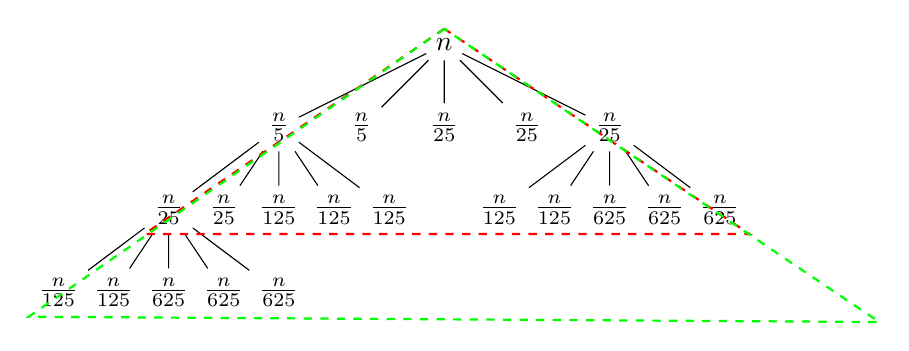
\begin{tikzpicture}
		[scale=.7,
		level 2/.style={sibling distance=1cm},]
		\node(root){$n$}
		child
		{
			node{$\frac{n}{5}$}
			child
			{
				node(5){$\frac{n}{25}$}
				child
				{
					node(1){$\frac{n}{125}$}
				}
				child
				{
					node{$\frac{n}{125}$}
				}
				child
				{
					node{$\frac{n}{625}$}
				}
				child
				{
					node{$\frac{n}{625}$}
				}
				child
				{
					node(2){$\frac{n}{625}$}
				}
			}
			child
			{
				node{$\frac{n}{25}$}
			}
			child
			{
				node{$\frac{n}{125}$}
			}
			child
			{
				node{$\frac{n}{125}$}
			}
			child
			{
				node{$\frac{n}{125}$}
			}
		}
		child
		{
			node{$\frac{n}{5}$}
		}
		child
		{
			node{$\frac{n}{25}$}
		}
		child
		{
			node{$\frac{n}{25}$}
		}
		child
		{
			node{$\frac{n}{25}$}
			child
			{
				node{$\frac{n}{125}$}
			}
			child
			{
				node{$\frac{n}{125}$}
			}
			child
			{
				node{$\frac{n}{625}$}
			}
			child
			{
				node{$\frac{n}{625}$}
			}
			child
			{
				node(4){$\frac{n}{625}$}
			}
		};
		\draw[red,thick,dashed](root.north)--(5.south west)--(4.south east)--(root.north);
		\node[xshift=10.3cm,yshift=-.25cm,name=f] at(1){};
		\draw[green,thick,dashed](root.north)--(1.south west)--(f.south east)--(root.north);
	\end{tikzpicture}
\end{center}
Osservando l'albero appena costruito notiamo subito l'esistenza di due percorsi che hanno velocità diverse: i sottoproblemi che vedono ridurre il proprio input di un venticinquesimo finiranno molto prima rispetto a quelli dove l'input si riduce, chiamata dopo chiamata, di solo un quinto. Per ricavare una stima asintotica dell'equazione di ricorrenza sarà necessario quindi studiare le stime dei due alberi di ricorsione $T_{1}(n) \leq T(n) \leq T_{2}(n)$ evidenziati rispettivamente in verde e rosso come mostrato in figura.
\begin{center}
	\begin{tblr}{hlines,vlines,cells={mode=math},row{1}={primary!80!white},row{1}={mode=text},colspec={cccccc}}
		\textbf{Livello} & $\mathbf{Input_{1}}$ & $\mathbf{Input_{2}}$&\textbf{Contributo locale} & \textbf{Rami} & \textbf{Costo livello} \\
		0 & n & n&4 & 1 & 4 \\
		1 & \frac{n}{5} & \frac{n}{25}  & 4 & 5 &   20 \\
		2 & \frac{n}{25} & \frac{n}{625}  &  4 & 25 & 100 \\
		3 & \frac{n}{125} & \frac{n}{15625} & 4 & 125&500 \\
		i & \frac{n}{5^{i}} & \frac{n}{5^{2i}} & 4 & 5^{i} & 5^{i} \cdot 4
	\end{tblr}
	\captionof{table}{}\label{tab:ex_recursion2}
\end{center}
Dalla tabella \ref{tab:ex_recursion2} si osserva che l'input dei sottoproblemi appartenenti al sottoalbero indotto $T_{1}$ segue un pattern definito dalla successione:
\begin{displaymath}
	\frac{n}{5^{h}}
\end{displaymath}
dove $h$ rappresenta l'altezza di $T_{1}$. Per determinare tale altezza bisogna determinare il livello in cui si raggiungono le foglie, ovvero il livello in cui, stando alla definizione dell'equazione di ricorrenza, vale:
\begin{displaymath}
	\frac{n}{5^{h}} \leq 1
\end{displaymath}
Risolvendo per $h$ si ottiene:
\begin{align*}
	\frac{n}{5^{h}} &\leq 1 \iff n \leq 5^{i} \implies h = \log_{5} n
\end{align*}
Il costo totale dell'albero $T_{1}$ si otterrà allora svolgendo la somma dei contributi livello per livello:
\begin{align*}
	T_{1}(n) &=\sum_{i=0}^{h} 4 \cdot 5^{i} = 4 \cdot \sum_{i = 1}^{h} 5^{i} = 4 \cdot \frac{i- 5^{h+1}}{1-5}\\
	&= \cancel{4} \frac{1-5^{h+1}}{\cancel{-4}} = - \bigl(1- 5^{\log_{5}n +1} \bigr)\\
	&= - \bigl(1 - 5 \cdot 5^{\log_{5}n}\bigr) = - \bigl(1 - 5 \cdot n \bigr) \\
	&= 5n -1 = \Theta(n)
\end{align*}
Svolgendo calcoli analoghi per il secondo albero si ottiene che l'altezza dell'albero $T_{2}$ vale $h= \frac{1}{2}\log_{5}n$. Quindi:
\begin{displaymath}
	T_{2}(n) = \sum_{i=0}^{h} 4 \cdot 5^{i} =  5 \sqrt{n}-1 =\Theta(\sqrt{n})
\end{displaymath}
Dato che le stime asintotiche dei due alberi non sono confrontabili possiamo concludere affermando di aver trovato un limite asintotico inferiore ed un limite asintotico superiore, ovvero:  $ \Omega(n)  \leq T(n) \leq O(\sqrt{n})$. \hfill \blacksquare

\begin{exsbox}
	Si risolva la seguente ricorrenza, calcolandone l'\textbf{andamento asintotico}:
	\begin{displaymath}
		T(n) = \begin{cases}
			1 & \text{se } n \leq 4\\
			8 \cdot T(\frac{n}{4}) + \sqrt{n} & \text{altrimenti}
		\end{cases}
	\end{displaymath}
\end{exsbox}

\begin{exsbox}
	Si risolva la seguente ricorrenza, calcolandone l'\textbf{andamento asintotico}:
	\begin{displaymath}
		T(n) = \begin{cases}
			1 & \text{se } n \leq 27\\
			3n^{2} \cdot T(\sqrt[3]{n}) + 2n^{3} & \text{altrimenti}
		\end{cases}
	\end{displaymath}
\end{exsbox}

\begin{exsbox}
	Si risolva la seguente ricorrenza, calcolandone l'\textbf{andamento asintotico}:
	\begin{displaymath}
		T(n) = \begin{cases}
			1 & \text{se } n \leq 2\\
			2 \cdot T(\sqrt[4]{n}) + \log(2n)& \text{altrimenti}
		\end{cases}
	\end{displaymath}
\end{exsbox}

\begin{exsbox}
	Si risolva la seguente ricorrenza, calcolandone l'\textbf{andamento asintotico}:
	\begin{displaymath}
		T(n) = \begin{cases}
			1 & \text{se } n \leq 1\\
			4 \cdot T(\frac{n}{2}) +n & \text{altrimenti}
		\end{cases}
	\end{displaymath}
\end{exsbox}

\subsection{Notazione asintotica}

\begin{exsbox}
	Si dimostri, \textbf{esplicitando il procedimento seguito nella sua interezza}, la verità o la falsità della seguente affermazione: \begin{displaymath}
		\log_{2}(n^{2n}) + n - \log_{2} n  = \Theta(\log_{2} n^{n})
	\end{displaymath}
	In caso affermativo, trovare le costanti che assicurano la validità della relazione.
\end{exsbox}

\paragraph{Svolgimento}
Per dimostrare la relazione possiamo avvalerci dell'equivalenza descritta dall'Equazione \ref{eq:theta2}. Posto $f(n) = \log_{2}(n^{2n}) + n - \log_{2} n$ e $g(n) = \log_{2} n^{n}$ si ha:
\begin{displaymath}
	f(n) = \Theta(g(n)) \iff \lim_{n \to +\infty} \frac{f(n)}{g(n)} = l \in \mathbb{R^{+}}
\end{displaymath}
Per dimostrare la veridicità della relazione è sufficiente quindi svolgere il limite di tale rapporto:
\begin{align*}
	\lim_{n \to +\infty} \frac{\log_{2}(n^{2n}) + n - \log_{2} n}{\log_{2} n^{n}} &= \lim_{n \to +\infty} \frac{2n \cdot \log_{2}(n) + n - \log_{2} n}{n \cdot \log_{2} n} & \text{\textcolor{gray}{Per le proprietà dei logaritmi}}\\
	&= \lim_{n \to +\infty} \frac{n \cdot \bigl(2 \cdot \log_{2}n + 1 - \frac{\log_{2} n}{n}\bigr)}{n \cdot \log_{2} n} & \text{\textcolor{gray}{Mettendo $n$ in evidenza}}\\
	&= \lim_{n \to +\infty} \frac{\cancel{n} \cdot \bigl(2 \cdot \log_{2}n + 1 - \frac{\log_{2} n}{n}\bigr)}{\cancel{n} \cdot \log_{2} n} & \text{\textcolor{gray}{Semplificando}}\\
	&= \lim_{n \to +\infty} \frac{2 \cdot \log_{2}n + 1 - \frac{\log_{2} n}{n}}{\log_{2} n}\\
	&= \lim_{n \to +\infty} \frac{\log_{2} n \bigl( 2 + \frac{1}{\log_{2 }n} - \frac{1}{n}\bigr)}{\log_{2} n}   & \text{\textcolor{gray}{Mettiamo in evidenza $\log_{2} n$}}\\
	&= \lim_{n \to +\infty} \frac{\cancel{\log_{2} n} \bigl(2 + \frac{1}{\log_{2}n} - \frac{1}{n}\bigr)}{\cancel{\log_{2} n}} & \text{\textcolor{gray}{Semplificando}} \\
	&= \lim_{n \to +\infty} 2 + \frac{1}{\log_{2}n} - \frac{1}{n} = 2 > 0
\end{align*}
Verificata la relazione, restano da trovare le costanti $n_{0}$, $c_{1}$ e $c_{2}$ che assicurano la relazione:
\begin{displaymath}
	\exists n_{0} \Bigl( \exists c_{1},c_{2}>0 \bigl( \forall n>n_{0} ( c_{1} < \frac{f(n)}{g(n)} < c_{2} ) \bigr) \Bigr)
\end{displaymath}
Riscriviamo la disequazione sostituendo gli effettivi valori per $f(n)$ e $g(n)$:
\begin{displaymath}
	c_{1} \leq \frac{\log_{2}(n^{2n}) + n - \log_{2} n}{\log_{2} n^{n}} \leq c_{2}
\end{displaymath}
che può essere riscritta come segue:
\begin{displaymath}
	c_{1} \cdot \log_{2} n^{n} \leq \log_{2}(n^{2n}) + n - \log_{2} n \leq c_{2} \cdot \log_{2} n^{n}
\end{displaymath}
La ricerca dell'esistenza delle costanti $n_{0}$, $c_{1}$ e $c_{2}$ equivale alla risoluzione delle due disequazioni nelle incognite $c_{1}$ e $c_{2}$:
\begin{displaymath}
	\begin{cases}
		c_{1} \cdot \log_{2} n^{n} \leq \log_{2}(n^{2n}) + n - \log_{2} n\\
		\log_{2}(n^{2n}) + n - \log_{2} n \leq c_{2} \cdot \log_{2} n^{n}
	\end{cases}
\end{displaymath}
L'obiettivo deve essere quello di ottenere una relazione indipendente dal valore di $n$.

\gbox{Suggerimento}{green-gradient-4}{
	All'interno di queste tipologie di dimostrazioni viene in aiuto il concetto di \textbf{maggiorazione} e \textbf{minorazione} delle funzioni che fanno largo utilizzo della proprietà transitiva.
	Supponiamo di voler dimostrare che $f(x) < A$, \textbf{maggiorare} una funzione $f(x)$ consiste nel trovare una funzione $g(x)$ possibilmente più semplice di $f$, tale che $|f(x)| \leq g(x)$ e tale che valga pure $g(x) < A$. Stando a quanto detto varrà la seguente catena di disuguaglianze:
	\begin{displaymath}
		f(x) \leq g(x) < A \implies f(x) < A
	\end{displaymath}
	che dimostra la relazione cercata. Dualmente per la minorazione di funzione.
	\marker{yellow!50}{yellow!20!black}{Se vogliamo maggiorare una frazione, dobbiamo maggiorare il numeratore e minorare il denominatore.}
}

Iniziamo studiando la prima delle due disequazioni. Si osserva che nel membro a destra esiste un unico termine sottrattivo. Osservando i grafici mostrati in Figura \ref{fig:log_linear} osserviamo che:
\begin{displaymath}
	\forall n \geq 0 (\log n < n)
\end{displaymath}
\begin{center}
	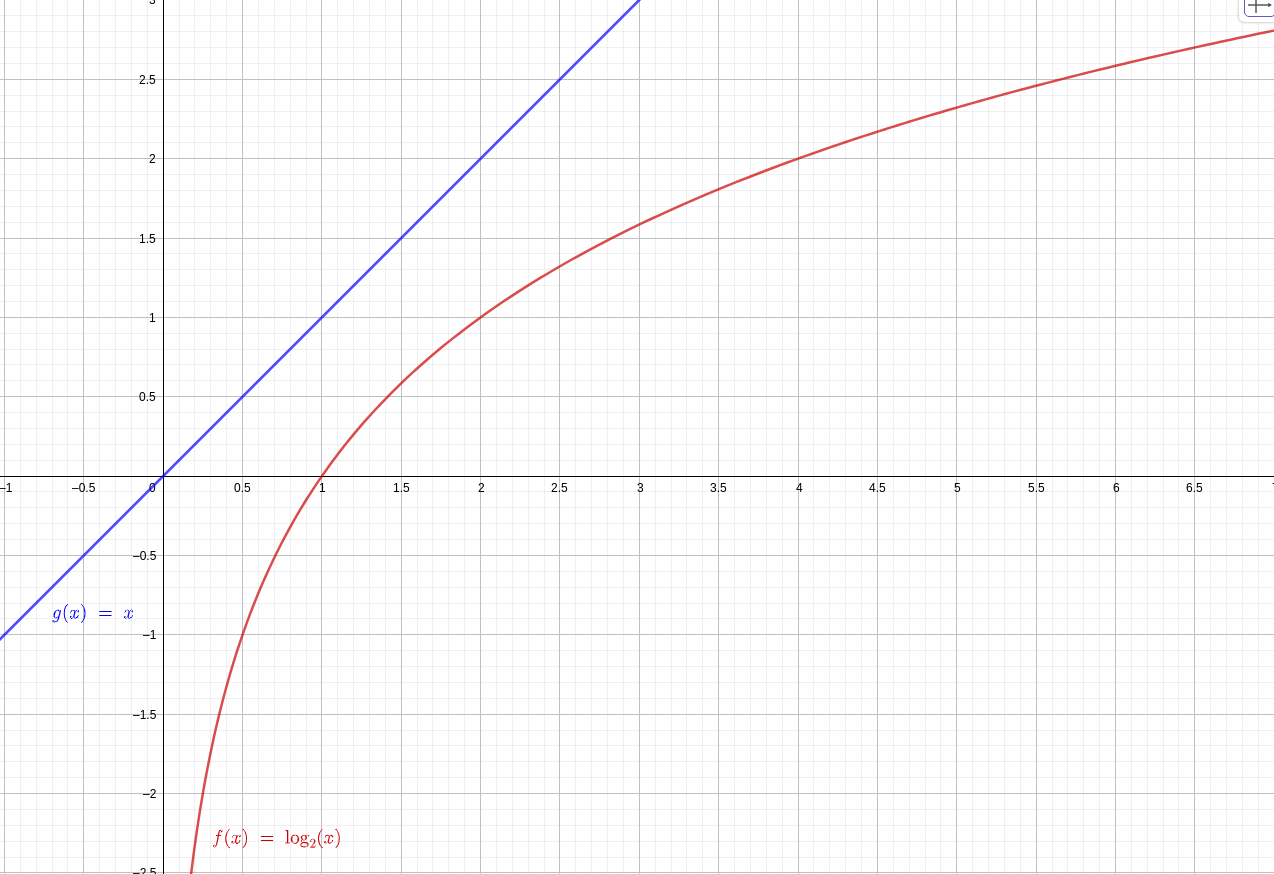
\includegraphics[scale=.2]{res/log_linear}
	\captionof{figure}{}\label{fig:log_linear}
\end{center}
Pertanto è possibile pensare di minorare la relazione sostituendo $n$ al termine sottrattivo presente ottenendo così una funzione più piccola\footnote{Sottraendo un qualcosa di più grande si ottiene l'effetto desiderato.}:
\begin{align*}
	c_{1} n \log_{2} n & \leq 2n \log_{2} + n -n = 2n \log_{2} < 2n \log_{2} n + n - \log_{2} n & \text{\textcolor{gray}{Minorando}}\\
	c_{1} &\leq \frac{2n \log_{2} n}{n \log_{2}n} \\
	c_{1} &\leq \frac{2 \cancel{n \log_{2} n}}{\cancel{n \log_{2} n}}\\
	c_{1} &\leq 2
\end{align*}
E otteniamo quindi $c_{1} = 2$. Nel svolgere la seconda disequazione possiamo sfruttare il fatto che, per ogni $n \geq 4$ vale: $n + \log_{2} n \leq n \log_{2} n$. Allora è possibile eseguire la seguente maggiorazione:
\begin{align*}
	2n \log_{2} n + n - \log_{2} n &< 2n \log_{2} n + n + \log_{2} n \leq 2n \log_{2} n + n \log_{2} n = 3n \log_{2} n \leq c_{2} n \log_{2} n
\end{align*}
da cui si ottiene $c_{2} \geq 3$ e quindi $c_{3}=3$. \hfill \blacksquare

\begin{exsbox}
	Si dimostri, \textbf{esplicitando il procedimento seguito nella sua interezza}, la verità o la falsità della seguente affermazione: se $f(n) = \Theta(\sqrt{g(n)})$ e $g(n)= \Theta((k(n))^{4})$ allora:
	\begin{displaymath}
		f(n) = \Theta((k(n))^{2})
	\end{displaymath}
	In caso affermativo, trovare le costanti che assicurano la validità della relazione.
\end{exsbox}
